\documentclass[a4paper,10pt,titlepage,pdfusetitle]{ltjsarticle}

% LINK
\usepackage{url}
\usepackage{hyperref}
\hypersetup{pdfborder={0 0 0.5}}

% 色の使用
\usepackage{xcolor}
\definecolor{mylinkcolor}{RGB}{3, 112, 145} %{65, 145, 3} % 色定義
\definecolor{linkcol}{RGB}{2, 106, 77} %{65, 145, 3} % 色定義
\hypersetup{
    colorlinks=true,
    citecolor=blue,
    linkcolor=linkcol,
    urlcolor=mylinkcolor % 定義された色
}
% HTML(#800000)色定義
\def\colH#1{\color[HTML]{#1}}


% 画像挿入
\usepackage{float}
\usepackage{graphicx}
\usepackage{svg} 

\usepackage{pst-barcode} 

% FONT
\usepackage{fontspec}
% FONT-WEIGHT 調整の指定
% \usepackage[haranoaji,deluxe,nfssonly,jis2004]{luatexja-preset}
\usepackage[haranoaji,deluxe]{luatexja-preset}

\usepackage{luatexja-otf} % UNICODE

% MACRO
\def\ocrb#1{\fontspec{ocrb7} {#1}}
\def\ocrbsmall#1{\fontspec{ocrb7} \fontsize{7}{7}{#1}\selectfont }



\usepackage{framed}

% DEFINE

% フォントサイズのマクロ定義が可能です。
\def\fsOCRB#1{\fontsize{#1pt}{14pt}\selectfont}

\def\fs#1#2{\fontsize{#1}{#2}\selectfont }
\def\bf#1{\textbf{#1}}
\newfontfamily\roboto{roboto}
% \newfontfamily\fRMono{RobotoMono-Regular}
\newfontfamily\fRMono{RobotoMono-Light}

% \newfontfamily\fOCRBRegular{ocrb-regular}
\newfontfamily\fOCRBRegular{OCRB-Regular}
   % UprightFont   = Calibri_Light.ttf,
   % ItalicFont    = Calibri_Light_Italic.ttf
\newfontfamily\fOCRBFree{OCRB-Free}
% \newfontfamily\fOCRBTestA{OCRB-TestA}
% \newfontfamily\fOCRBTestB{OCRB-TestB}
% \newfontfamily\fOCRBTestC{OCRB-TestC}
% \newfontfamily\fOCRBTestD{OCRB-TestD}
% \newfontfamily\fOCRBTestE{OCRB-TestE}


\def\bs{\textbackslash}

\title{\Huge 日本語書籍用ISBNバーコードの作成\\ \huge Template with Lua\LaTeX{}\vspace{10mm}\\ \Large\lbrack\ pst-barcode\ \rbrack\vspace{100mm}}

\author{\href{https://github.com/ru-museum?tab=repositories}{ru\_museum}: GitHub)}
\date{\today}

\begin{document}
\thispagestyle{empty}

\maketitle

\setcounter{tocdepth}{2}
\clearpage
\thispagestyle{empty}
\tableofcontents
\newpage

\section{日本語書籍用ISBNバーコードの制作}   

\begin{itemize}

  \item 日本で出版される書籍には、一般的に「日本図書コード\footnote{ISBNコード(国際標準図書番号)に分類と価格表記を付加した日本独自のもの。\\例:ISBN978-4-06-278761-1 C2055 ¥3000E}」と「書籍JANコード\footnote{日本図書コード(分類番号及び価格を含めたもの)を組み入れた国内での出版流通に利用されるもの。}」とが表記されることとなっています。
  
  \item 「書籍 JAN コード」には、国際標準図書番号であるISBNコード(978-)と日本語書籍で使用されている独自の日本図書コード(192-)とがあります。
  
  \item 共にエンコード方式は {\colH{800000}EAN-13}\footnote{EAN(European Article Number)。国際標準となっているバーコード変換様式。}ですが、日本語書籍で使用されている「日本図書コード」としての ISBN バーコードは、国際標準 ISBN バーコードとはその表記方式が異なっています\footnote{セパレータの有無等。}。\vspace{-4mm}\\

\hspace{11mm}書籍JANコード(2段組) \hspace{10mm}国際標準 ISBN コード\vspace{-4mm}
\begin{figure}[h]  
\setlength{\unitlength}{0.14in} 
\centering                      
\begin{picture}(62,15) 
\put(6,11){\psbarcode{9784003261842}{height=0.45 width=1.28}{ean13}}  
\put(6,10){{\fontspec{ocrb7}9784003261842}}
\put(6,6){\psbarcode{1920197009404}{height=0.45 width=1.28}{ean13}}  
\put(6,5){{\fontspec{ocrb7}1920197009404}}  
 
\put(18,7.7){ 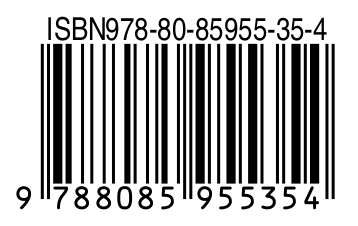
\includegraphics[width=4cm,angle=0]{./images/ean-13-sample.png}} 
\end{picture}  
\end{figure}\vspace{-20mm}\relax  
  \item \LaTeX{} では日本図書コードに用いるISBNバーコードを作成出来るパッケージは用意されていません。\\
  ここではTexLive付属\footnote{/usr/share/texlive/texmf-dist/tex/latex/pst-barcode(linux: Debian)}の \textbf{\colH{800000}pst-barcode} をカスタマイズし利用します。\vspace{-1em}    
\end{itemize}

\section{表記・印刷の規格} 

\begin{itemize}
  \item 書籍 JAN コードの表記・印刷位置は厳密に定められています。\footnote{\href{https://isbn.jpo.or.jp/doc/08.pdf}{「ISBNコード/日本図書コード/書籍JANコード利用の手引き」}\\
\hspace{2em}(2010年版 : 日本図書コード管理センター)}\vspace{-6mm}

\end{itemize}

\subsection{サイズ}\vspace{-8mm} 

{\begin{figure}[H]
\centering
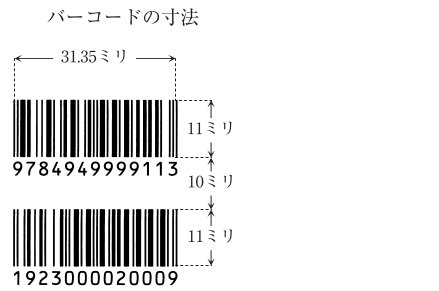
\includegraphics[width=8cm,angle=0]{./images/isbn-layout01.png}
\caption{サイズ規格}\vspace{-6mm} 
\end{figure}

\subsection{表記位置}\vspace{-6mm} 
\begin{figure}[H]
\centering
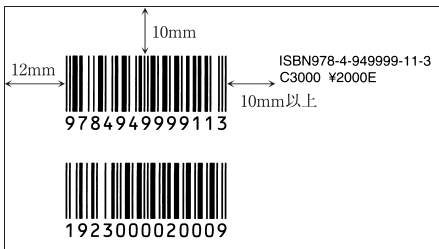
\includegraphics[width=8cm,angle=0]{./images/isbn-layout02.png}
\caption{位置規格(裏表紙左上の場合)} 
\end{figure}

\section{作成手順}   

\subsection{作業環境}

\begin{itemize}
  \item[] Debian GNU/Linux\\
  TexLive バージョン (2021.20220204-1) / Debianパッケージ\\
LuaLatex
\end{itemize}
\vspace{-4mm}

\subsection{パッケージpst-barcode}
\begin{itemize}
  \item TexLive 付属のパッケージ\textbf{pst-barcode}\footnote{他にも幾らかバーコード用パッケージが存在しますが、「書籍JANコード」として改造の行えるものはありませんでした。}を使用します。\\
{\fRMono
\bs usepackage\{{\colH{800000}pst-barcode}\}\\
 begin\{document\}\\
\quad\bs psbarcode\{9784003261842\}\{height=0.45 width=1.28\}\{ean13\}
}\vspace{1mm}
  \item pst-barcodeでは「書籍JANコード」の2段組の各々を直接表記することは出来ません。\\
  そこで、pst-barcode側で\textbf{バーコード部分のみを生成しISBN番号部分は非表示}とし、番号部分をlatex側で補完及び調整を行っています。
\end{itemize}
\vspace{-4mm}

\subsection{フォントの指定}
\begin{itemize}
  \item ISBNコード表記では特別な{\colH{800000}OCRB フォント}\footnote{\roboto{5 OCRB \textbf{フォントの使用}}を参照。}が使われます。\\
\textbf{記述例:}\fRMono{\{\bs fontspec\{ocrb7\}9784003261842\}}\\
\textbf{表示例:}\hspace{2mm}{\fontspec{ocrb7}9784003261842}\\
\end{itemize}
\vspace{-10mm}
  
\subsection{サイズ(高さ、幅)の指定}\vspace{-2mm}

\begin{itemize}
  \item height={\colH{800000}n} width={\colH{800000}n} で指定します。\\
  {\colH{800000}n} は数値、オプションの設定要素間は{\colH{800000}半角空白}で区切られます。\\
\fRMono{
\bs psbarcode\{9784003261842\}\{height=0.45\,{\colH{800000}␣}\,width=1.28\}\{ean13\}
}\vspace{-8mm}
\end{itemize}

\newpage

\subsection{表示}\vspace{-2mm}
\begin{itemize}
  \item[] 
{\fRMono
\{\bs begin\{picture\}(0,50)({\colH{800000}-10},{\colH{800000}20})\\
\bs psbarcode\{9784003261842\}\{{\colH{800000}height=0.45 width=1.28}\}\{ean13\}\\
\bs end\{picture\}\}\bs quad{\colH{800000}\bs vspace\{4.6mm\}}\\ 
{\colH{800000}\bs hspace\{3mm\}}\{\bs fontspec\{ocrb7\}9784003261842\}\\ 
\bs vspace\{2mm\}\vspace{-10mm}
}

{\begin{picture}(0,50)(-10,20)
\psbarcode{9784003261842}{height=0.45 width=1.28}{ean13}
\end{picture}}\quad\vspace{4.6mm}\\
\hspace{3mm}{\fontspec{ocrb7}9784003261842}\\
\vspace{2mm}
\end{itemize}
\vspace{-12mm}

\begin{enumerate}
  \item \bf{各項目の表示位置調整}
\begin{itemize}
  \item バーコードとISBN番号との左右上下のズレは、ISBN番号前後の{\colH{800000}\bs vspace}と{\colH{800000}\bs hspace}、或いは{\colH{800000}\bs picture}及び{\colH{800000}\bs put}のオフセット数値を替え正確な位置を調整します。
  \item オフセット値はマイナス値となることもあります。\\
    \quad\bs begin\{picture\}( x 方向(横)の長さ, y 方向(縦)の長さ )( x のオフセット, y のオフセット)\\ 
    \quad\bs put( x のオフセット, y のオフセット)
  \item x及びyの各移動方向は{\colH{800000}正負逆向き}となっていますので注意して下さい。
\end{itemize}


{\renewcommand{\arraystretch}{1.6}%
\begin{table}[h]
\begin{center}
\begin{tabular}{|c|c|c|c|}
\hline
\multicolumn{2}{|c|}{\roboto\bf x のオフセット} & \multicolumn{2}{|c|}{\roboto\bf y のオフセット}\\[5pt]
\hline
n > 0 & n < 0 &  n > 0 & n < 0\\[5pt]
\hline
\raisebox{-0.8ex}{\includesvg[width=1.2em,angle=0]{./icons/west_black.svg}} & \raisebox{-0.8ex}{\includesvg[width=1.2em,angle=0]{./icons/east_black.svg}} & 
\raisebox{-0.8ex}{\includesvg[width=1.2em,angle=0]{./icons/south_black.svg}} & \raisebox{-0.8ex}{\includesvg[width=1.2em,angle=0]{./icons/north_black.svg}}\\[5pt]
\hline
\end{tabular}
\caption{xとyのオフセット設定値(n)と移動方向}
\end{center}
\end{table}
}
 
  \item \bf{表示例:}
\begin{verbatim}
\begin{picture}(0,0)(-40,120)
\put(-33,76){\psbarcode{9784003261842}{height=0.45 width=1.28}{ean13}}  
\put(-34,66){{\fontspec{ocrb7}9784003261842}}  
\put(-33,13){\psbarcode{1920197009404}{height=0.45 width=1.28}{ean13}}  
\put(-34,3){{\fontspec{ocrb7}1920197009404}}  
\put(92,100){\fontspec{ocrb7}ISBN4-00-326184-4}  
\put(92,78){\fontspec{ocrb7}C0197 \gtfamily{\bfseries¥}940E}  
\put(92,46){\fs{12}{12}{\gtfamily{\mdseries 定価(本体 {\fontspec{Inter-Medium}940}円+税)}}}
\end{picture}
\end{verbatim}

\newpage

\begin{picture}(0,0)(-40,120)
\put(-33,76){\psbarcode{9784003261842}{height=0.45 width=1.28}{ean13}}  
\put(-34,66){{\fontspec{ocrb7}9784003261842}}  
\put(-33,13){\psbarcode{1920197009404}{height=0.45 width=1.28}{ean13}}  
\put(-34,3){{\fontspec{ocrb7}1920197009404}}  

\put(92,100){\fontspec{ocrb7}ISBN4-00-326184-4}  
\put(92,78){\fontspec{ocrb7}C0197 \gtfamily{\bfseries¥}940E}  
\put(92,46){\fs{12}{12}{\gtfamily{\mdseries 定価(本体 {\fontspec{Inter-Medium}940}円+税)}}}
\end{picture}  
\end{enumerate}
\vspace{40mm}


\section{定期刊行物コード(雑誌)}

\begin{itemize}
  \item JANコードに準拠する13桁(左)は{\colH{800000}ean13}、価格を表現する5桁のアドオンコード(右)は{\colH{800000}ean5}によりエンコードされています。
  \item シンボルの高さは基本12mmですが、製本時の「断ち落とし」に備え15mm以上が必要です。\\
  通常多くは15mmで表示されています(図3は裁断された例です)。
  \item 各部品の位置調整は {\gtfamily{\mdseries 3 作成手順}}を参照して下さい。
\end{itemize}
\vspace{-6mm}

% 定期刊行物コード
\begin{picture}(0,0)(76,120)
\put(92,100){\gtfamily{\mdseries 雑誌} {\fontspec{roboto}06615—08}}  
\end{picture}  

\begin{pspicture}(-34mm,18mm)
\psbarcode{4910066150853}{height=0.61 width=1.24}{ean13}
\end{pspicture}
% SPACE: 2.31mm
\begin{pspicture}(-32.6mm,18mm)
\psbarcode{00093}{height=0.61 width=0.66}{ean5}
\end{pspicture}

\begin{picture}(0,0)(-157,48)
\put(92,100){\fontspec{ocrb7}4910066150853}  
\end{picture}  
\begin{picture}(0,0)(-211.4,59)
\put(92,100){\fontspec{ocrb7}00093}  
\end{picture}  
\vspace{-6mm}

\begin{figure}[H]
\centering
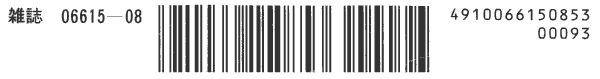
\includegraphics[width=11.6cm,angle=0]{./images/barcode-magazine0001.png}
\caption{定期刊行物コード(雑誌)表示例} 
\end{figure}
\vspace{-10mm}

\section{FONT-WEIGHT の調整}

\subsection{luatexja-preset で deluxe を設定} 
\fRMono{\textbackslash usepackage[{\colH{800000}deluxe}]\{luatexja-preset\}}

\subsection{フォントの字体指定}\vspace{-10mm} 
\begin{table}[H]
\begin{tabular}{llll}
\textbf{コマンド} & \textbf{字体指定} & \textbf{表示例} & \textbf{フォント}\\
\hline
   & 標準 & {\fontspec{HaranoAjiMincho-Regular} 戦争と平和 4} & HaranoAjiMincho-Regular\\
  \textbackslash textbf & 太字 & \textbf{\fontspec{HaranoAjiMincho-Regular} 戦争と平和 4} & HaranoAjiMincho-Regular\\
  \textbackslash ltseries & 細字 & \ltseries{\fontspec{HaranoAjiMincho-Bold} 戦争と平和 4} & HaranoAjiMincho-Bold\\
  \textbackslash mdseries & 中字 & \mdseries{\fontspec{NotoSerifJP-Regular} 戦争と平和 4} & NotoSerifJP-Regular\\
  \textbackslash bfseries & 太字 & \bfseries{\fontspec{NotoSerifJP-Bold} 戦争と平和 4} & NotoSerifJP-Bold\\
\end{tabular}
\end{table}
\vspace{-6mm}

\begin{itemize}
  \item その他、TexLive同梱のフォントやシステムにインストールされたもの、独自にインストールしたフォントも利用可能です。
\end{itemize}
\vspace{-6mm}

\section{OCRB フォントの使用}
\begin{itemize}
  \item \href{https://imagers.co.jp/contents/1537/}{OCRB フォントとは}ISOで規格化された国際規格となっています。
  \item \href{https://ctan.org/pkg/ocr-b-outline}{ocr-b-outline – OCR-B fonts in Type 1 and OpenType}(CTAN)\\
{\fs{9}{9} ※ 従来の .mf フォントは LuaLaTeX では使用出来ませんので OTF を使用します。}
\end{itemize}
\vspace{-6mm}

\subsection{インストール方法}
\begin{itemize}
  \item リンク先よりダウンロード・解凍し以下のフォルダに配置します。\\
/usr/share/texlive/texmf-dist/fonts/opentype/public/\textbf{\colH{800000}ocr-b-outline}\vspace{-2mm}\\
{\fs{9}{6}
\begin{verbatim}
ocr-b-outline
 ├─ fontforge
 ├─ map
 ├─ opentype
 │  ├── ocrb5.otf
 │  ├── ocrb6.otf
 │  ├── ocrb7.otf
 │  ├── ocrb8.otf
 │  ├── ocrb9.otf
 │  └── ocrb10.otf
 └─ type1
\end{verbatim}\vspace{-5mm}
}
\end{itemize}

\subsection{ISBN番号表示例}\vspace{-2mm}
\begin{itemize}
  \item[]
\fRMono{\{{\colH{800000}\bs ocrb} ISBN978-4-06-278761-1\}}\\
\quad{\ocrb ISBN978-4-06-278761-1}\\
\fRMono{\{{\colH{800000}\bs ocrbsmall}\bs quad ISBN978-4-06-278761-1\}}\\
{\ocrbsmall\quad ISBN978-4-06-278761-1}\vspace{-6mm}\\

\fRMono{\{\bs fontspec\{{\colH{800000}ocrb7}\}ISBN978-4-06-278761-1\}}\\
\quad{\fontspec{ocrb7}ISBN978-4-06-278761-1}\\
\fRMono{\{\bs fontspec\{{\colH{800000}ocrb9}\}ISBN4-00-326184-4 C0197 \bs gtfamily\{\bs bfseries¥\}940E\}}\\
\quad{\fontspec{ocrb9}ISBN4-00-326184-4 C0197 \gtfamily{\bfseries¥}940E}\\
\end{itemize}
\vspace{-12mm}



\subsection{「{\jfontspec{OCRB-Regular} \UTF{00A5}}(¥)」円マーク文字について}\vspace{-2mm}

\begin{itemize}

  \item CTAN版フォントには「{\jfontspec{OCRB-Regular} \UTF{00A5}}」マークは 収録されていません。\\使用に際しては{\colH{800000}円記号(¥)を太字化}することで補完出来ます。\\
その他の方法は、\bf{\roboto 5.3.1〜3}の\bf{「{\jfontspec{OCRB-Regular} \UTF{00A5}}」マーク使用例}を参照して下さい。
  
\vspace{-2mm}
\begin{figure}[H]
\centering
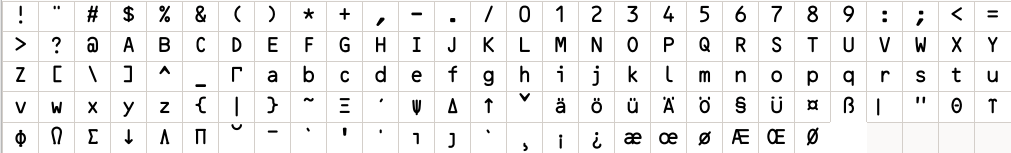
\includegraphics[width=14cm]{./images/ocrb-ttf01.png}
\caption{ocrb7(CTAN)} 
\end{figure}
\vspace{-6mm}

  \item 「{\jfontspec{OCRB-Regular} \UTF{00A5}}」マークを収録しているOCRBフォントには各社提供のものがあります\footnote{Microsoft社のものはWindows OSに付属しています。\\OCRB Regularはフリーフォントとして公開されていますがライセンスはAdobe社となっています。\\入手先:\href{https://freefonts.co/fonts/ocrb-regular}{OCRB Regular // Free Fonts}\\利用に際しては場合により著作権問題が生じることがありますので注意が必要です。}。

\vspace{-2mm}
  
\begin{figure}[H]
\centering
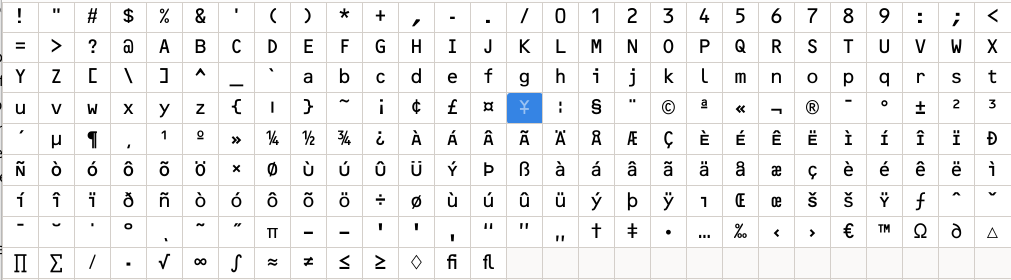
\includegraphics[width=14cm]{./images/ocrb-ttf-ms2.png}
\caption{OCRB.TTF(Microsoft Windows 付属)} 
\end{figure}
\vspace{-6mm}

\begin{figure}[H]
\centering
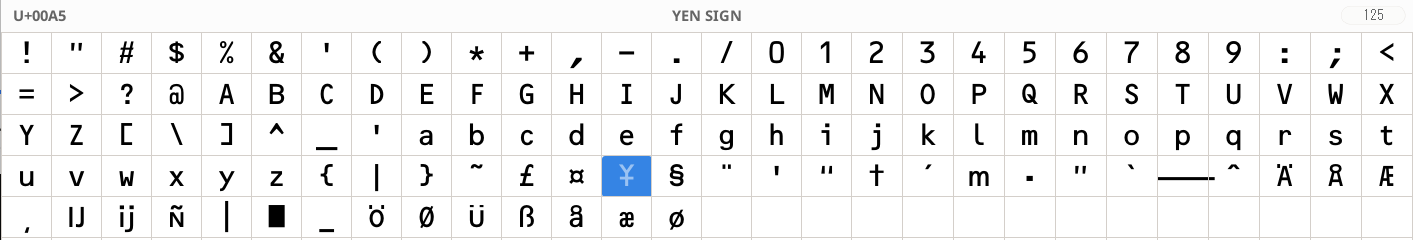
\includegraphics[width=14cm]{./images/ocrb-regular02.png}
\caption{OCRB Regular.OTF( Free Fonts)} 
\end{figure}

\end{itemize}

\subsubsection{「{\jfontspec{OCRB-Regular} \UTF{00A5}}」マーク使用例1:フォントA}

\begin{itemize}
  \item ここでは公開されているフリーフォントOCRB-Regularを使用した例を示します。\\
  \href{https://freefonts.co/fonts/ocrb-regular}{OCRB Regular // Free Fonts}\quad https://freefonts.co/fonts/ocrb-regular
\begin{enumerate}
  \item フォントのインストール\\
  /usr/share/texlive/texmf-dist/fonts/opentype/{\colH{800000}ocrb-regular}/{\colH{800000}OCRB-Regular.otf}\\
{\colH{800000}【注】}フォント名「OCRB Regular.otf」を「OCRB{\colH{800000}-}Regular.otf」と変更します。\\
\hspace{24pt}LuaLaTeXではフォルダへ保存されると次回から認識反映されます。
  \item フォントの指定\\
\bs {\colH{800000}jfontspec}\{OCRB-Regular\} \% fontspecではエラーとなります。
  \item ユニコードの使用\\
  \bs UTF\{<unicode>\} \% \bs usepackage\{luatexja-otf\} が必要
  \item 記述と表記\\
記述例:\fRMono{\{\bs jfontspec\{{\colH{800000}OCRB-Regular}\} \bs UTF\{{\colH{800000}00A5}\}\}}\\
表記例:{\fontspec{ocrb7}C0197 {\jfontspec{OCRB-Regular} \UTF{00A5}}\hspace{-2pt}940E}\\
\end{enumerate}
\end{itemize}
\vspace{-10mm}

\subsubsection{「{\jfontspec{OCRB-Regular} \UTF{00A5}}」マーク使用例2:フォントB}

\begin{itemize}
  \item {\colH{800000}著作権問題}を忌避する為、自作OCRBフォント(ttf)を使用した例を示します。\\
    OCRB文字セットは{\colH{388ED9}STANDARD ECMA-11}\footnote{\href{https://ecma-international.org/wp-content/uploads/ECMA-11\_3rd\_edition\_march\_1976.pdf}{STANDARD ECMA-11 for The Alphanumeric character set OCR-B for optical recognition. 3rd Edition 1976}\\https://ecma-international.org/wp-content/uploads/ECMA-11\_3rd\_edition\_march\_1976.pdf\\参考:「\href{https://kikakurui.com/x9/X9001-1976-01.html}{日本工業規格 JISX 9001-1976 光学式文字認識のための字形(英数字)}」\\\hspace{24pt}kikakurui.com: https://kikakurui.com/x9/X9001-1976-01.html}に準拠しています。
\begin{enumerate}
  \item フォントのインストール\\
  添付のフォント(fonts/OCRB-Free.ttf)を以下のフォルダを作成し保存します。\\
/usr/share/texlive/texmf-dist/fonts/truetype/{\colH{800000}ocrb}/{\colH{800000}OCRB-Free.ttf}\\
{\colH{800000}【注】}OCRB-Freeフォントは開発中ですので「{\jfontspec{OCRB-Free} \UTF{00A5}}」マークのみを収録しています。\\
\hspace{24pt}LuaLaTeXではフォルダへ保存されると次回から認識反映されます。
  \item フォントの指定\\
\bs {\colH{800000}jfontspec}\{OCRB-Free\} \% fontspecではエラーとなります。
  \item ユニコードの使用\\
  \bs UTF\{<unicode>\} \% \bs usepackage\{luatexja-otf\} が必要
  \item 記述と表記\\
記述例:\fRMono{\{\bs jfontspec\{{\colH{800000}OCRB-Free}\} \bs UTF\{{\colH{800000}00A5}\}\}}\\
\hspace{37pt}\fRMono{\{\bs fontspec\{ocrb7\}C0197 \{\bs jfontspec\{{\colH{800000}OCRB-Free}\} \bs UTF\{{\colH{800000}00A5}\}\}940E\}}\\
表記例:10pt:{\fs{10}{20}{\fontspec{ocrb7}C0197 {\jfontspec{OCRB-Free} \UTF{00A5}}940E}}\\
\hspace{37pt}12pt:{\fs{12}{20}{\fontspec{ocrb7}C0197 {\jfontspec{OCRB-Free} \UTF{00A5}}940E}}\vspace{-2mm}\\
\hspace{37pt}20pt:{\fs{20}{20}{\fontspec{ocrb7}C0197 {\jfontspec{OCRB-Free} \UTF{00A5}}940E}}  
\end{enumerate}
\end{itemize}

\subsubsection{「{\jfontspec{OCRB-Regular} \UTF{00A5}}」マーク使用例3:SVG}
\begin{itemize}
  \item ここでは{\colH{800000}著作権問題を考慮した場合}を想定しSVG画像を使用した例を示します。\\
\vspace{-2mm}
\begin{enumerate}
  \item ライブラリの呼び込み\\
  \bs usepackage\{svg\}\\
  ・画像の読込にはInkscapeのインストールが必要です。  
  \item SVG画像 \\
      画像は添付の./images/{\colH{800000}ocrb-yen.svg}を使用します。\\
     ・OCRB文字セットは\href{https://ecma-international.org/wp-content/uploads/ECMA-11\_3rd\_edition\_march\_1976.pdf}{STANDARD ECMA-11}(\roboto 脚注*10参照)に準拠しています。      
  \item 記述と表記\\
記述例:\fRMono{\bs includesvg[width=12pt]\{./images/ocrb-yen.svg\}}\\
\hspace{36pt}・widthにより大きさを設定します(in, pt, mm 他)。\\

\begin{table}[h]
\begin{center}
\begin{tabular}{lllllll}
\hspace{-6pt}\bf{設定値}: & \bf{2mm} & \bf{4mm} & \bf{12pt} & \bf{0.2in} & \bf{6mm}\\
 & \hspace{10pt}\includesvg[width=2mm]{./images/ocrb-yen.svg} & 
\hspace{8pt}\includesvg[width=4mm]{./images/ocrb-yen.svg} & 
\hspace{6pt}\includesvg[width=12pt]{./images/ocrb-yen.svg} & 
\hspace{6pt}\includesvg[width=0.2in]{./images/ocrb-yen.svg} & 
\hspace{4pt}\includesvg[width=6mm]{./images/ocrb-yen.svg}\\
\hline
\end{tabular}
\caption{表記例}
\end{center}
\end{table}
\vspace{-4mm}
表記例:{\fontspec{ocrb7}C0197 \includesvg[width=5.4pt]{./images/ocrb-yen.svg}\hspace{1pt}940E}  

\end{enumerate}
\end{itemize}

\section{作成例テンプレート}
\begin{itemize}
  \item 作成例テンプレートは同梱の\href{samples-isbn-barcode-ja.pdf}{書籍JANコード サンプル集}samples-isbn-barcode-ja.pdfをご覧下さい。
  \item 利用の為のサンプルコードは同名の\href{samples-isbn-barcode-ja.tex}{書籍JANコード サンプル集}samples-isbn-barcode-ja.texをご覧下さい。
  
\end{itemize}


\end{document}

